\section{Results}
\label{sec:results}

% Every number below comes from results/summary/v2/analysis.json, produced by
% eval/analyze.py over the 5-seed v2 run (and results/summary/v2c for the
% ConvNeXt check, via eval/backbone.py); tables/*.tex are generated by them.

\subsection{Predictors are comparable on accuracy}
Table~\ref{tab:main} reports accuracy and probabilistic quality on the seen test
expressions. The deterministic, evidential, and MC-dropout predictors are within
seed noise of each other (CCC $0.712$--$0.720$, std $\approx0.01$); the Gaussian
head is consistently weaker ($0.693$), and ensembling five seeds adds about
$0.01$ for either head. Our evidential model reaches CCC $0.829$ on valence and
$0.610$ on arousal. For context, the AffectNet authors' baseline reports
$0.541$ and $0.450$ on their test set~\cite{mollahosseini2017affectnet}, and
EmoNet~\cite{toisoul2021estimation} reports $0.82$ and $0.75$ on a cleaned test
set. These comparisons are indicative only, since the partitions differ (see
Section~\ref{sec:experiments}). The point is that the coverage results below rest
on a predictor of representative strength. On proper scores, the evidential head
has the best NLL ($-0.067$) and the evidential ensemble the best CRPS
($0.135$). Calibration error disagrees: the ensembles have the \emph{worst} ECE
($0.043$--$0.044$, against $0.022$--$0.027$ for single models) despite better
proper scores, a reminder that ECE alone does not rank predictors.

\begin{table}[h]
  \centering\small
  \resizebox{\linewidth}{!}{\begin{tabular}{lccccccc}
\toprule
Method & CCC-V$\uparrow$ & CCC-A$\uparrow$ & RMSE$\downarrow$ & NLL$\downarrow$ & CRPS$\downarrow$ & ECE$\downarrow$ & AURC$\downarrow$ \\
\midrule
Deterministic & 0.822$_{\pm.008}$ & 0.602$_{\pm.011}$ & 0.269$_{\pm.003}$ & -- & -- & -- & -- \\
Gaussian & 0.807$_{\pm.009}$ & 0.579$_{\pm.022}$ & 0.274$_{\pm.003}$ & 0.006$_{\pm.013}$ & 0.144$_{\pm.002}$ & \textbf{0.022}$_{\pm.011}$ & 0.041$_{\pm.001}$ \\
Evidential & 0.829$_{\pm.006}$ & 0.610$_{\pm.010}$ & 0.270$_{\pm.003}$ & \textbf{-0.067}$_{\pm.015}$ & 0.138$_{\pm.002}$ & 0.026$_{\pm.010}$ & 0.039$_{\pm.002}$ \\
MC-dropout & 0.829$_{\pm.006}$ & 0.610$_{\pm.011}$ & 0.270$_{\pm.003}$ & 0.002$_{\pm.017}$ & 0.138$_{\pm.002}$ & 0.027$_{\pm.010}$ & 0.039$_{\pm.002}$ \\
Gaussian ens. & 0.817 & 0.595 & 0.266 & -0.031 & 0.139 & 0.044 & 0.038 \\
Evidential ens. & \textbf{0.838} & \textbf{0.624} & \textbf{0.262} & -0.053 & \textbf{0.135} & 0.043 & \textbf{0.036} \\
\bottomrule
\end{tabular}
}
  \caption{Accuracy and probabilistic quality on seen test expressions.
  Mean$_{\pm\text{std}}$ over five seeds; ensembles combine the five seeds.
  NLL and CRPS are proper scores (lower is better).}
  \label{tab:main}
\end{table}

\subsection{Per-axis intervals under-cover the VA point}
Table~\ref{tab:coverage} compares the three conformal constructions on top of
every predictor. With per-axis intervals, joint coverage is $0.853$--$0.861$,
four to five points below nominal, for every predictor and with seed std below
$0.01$: the shortfall is systematic, not noise. The max-score region restores it
($0.917$--$0.930$), as does Bonferroni ($0.922$--$0.941$), but the max-score
region is smaller in every case: by $11\%$ for the evidential model ($1.39$
versus $1.57$), $13\%$ for the evidential ensemble, $7\%$ for the Gaussian head,
and $3\%$ for the deterministic one. The saving grows with the quality of
$\hat\sigma$, as expected, since a constant scale leaves no dependence between
the normalised residuals for the max-score to exploit beyond that of the raw
residuals.

The gap is also uneven across expressions (Figure~\ref{fig:per_emotion}). Under
per-axis intervals, six of the seven seen expressions are below nominal for the
evidential model, and \emph{sad} is covered least ($0.836$); for the
deterministic model it falls to $0.784$. The max-score region raises the
worst seen expression to $0.905$ for the evidential model, but only to $0.868$
for the deterministic one: with a constant scale, the region has the same shape
for every face, so it cannot widen where errors are larger. Learned
uncertainty is what makes group coverage close to uniform. Coverage above
nominal on the overall test set reflects the label shift between the
class-balanced calibration split and the imbalanced test split, which
over-represents \emph{happy}, an expression with narrow residuals.

\begin{table}[h]
  \centering\small
  \resizebox{\linewidth}{!}{\begin{tabular}{lcccccccc}
\toprule
 & \multicolumn{2}{c}{Per-axis} & \multicolumn{2}{c}{Bonferroni} & \multicolumn{2}{c}{Max-score (ours)} & \multicolumn{2}{c}{Worst / Shift (ours)} \\
Method & Joint & Area & Joint & Area & Joint & Area & Worst & Shift \\
\midrule
Deterministic & 0.860$_{\pm.005}$ & 0.991$_{\pm.015}$ & 0.922$_{\pm.005}$ & 1.561$_{\pm.028}$ & 0.920$_{\pm.005}$ & 1.517$_{\pm.023}$ & 0.868$_{\pm.014}$ & 0.809$_{\pm.047}$ \\
Gaussian & 0.853$_{\pm.007}$ & 0.792$_{\pm.021}$ & 0.929$_{\pm.007}$ & 1.281$_{\pm.048}$ & 0.921$_{\pm.005}$ & 1.186$_{\pm.039}$ & 0.879$_{\pm.019}$ & 0.879$_{\pm.066}$ \\
Evidential & 0.861$_{\pm.003}$ & 0.826$_{\pm.018}$ & 0.941$_{\pm.003}$ & 1.567$_{\pm.057}$ & 0.930$_{\pm.005}$ & 1.388$_{\pm.048}$ & \textbf{0.905}$_{\pm.007}$ & 0.920$_{\pm.023}$ \\
MC-dropout & 0.860$_{\pm.004}$ & 0.822$_{\pm.016}$ & 0.941$_{\pm.003}$ & 1.566$_{\pm.052}$ & 0.929$_{\pm.004}$ & 1.376$_{\pm.049}$ & 0.904$_{\pm.007}$ & 0.920$_{\pm.023}$ \\
Gaussian ens. & 0.855 & 0.717 & 0.928 & 1.124 & 0.917 & \textbf{1.024} & 0.883 & 0.924 \\
Evidential ens. & 0.860 & 0.721 & 0.937 & 1.348 & 0.924 & 1.178 & \textbf{0.905} & 0.934 \\
\bottomrule
\end{tabular}
}
  \caption{Conformal regions at nominal $90\%$, calibrated on validation. Joint:
  fraction of seen test faces whose true VA point lies in the region. Area: mean
  region area in VA units. Worst: lowest joint coverage across the seven seen
  expressions. Shift: joint coverage on corrupted test images, with the quantile
  calibrated on clean data.}
  \label{tab:coverage}
\end{table}

\begin{figure}[t]
  \centering
  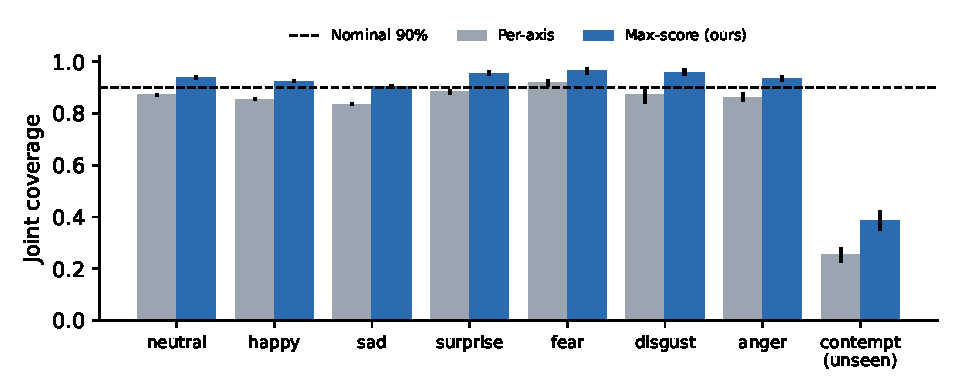
\includegraphics[width=\linewidth]{tables/per_emotion.pdf}
  \caption{Joint coverage of the true VA point per expression (evidential head,
  nominal $90\%$, dashed). Per-axis intervals under-cover most seen expressions;
  the max-score region lifts every seen expression to near or above nominal.
  Contempt, absent from training and calibration, is far below nominal under
  both.}
  \label{fig:per_emotion}
\end{figure}

\subsection{Unseen expressions break every guarantee}
On \emph{contempt}, which no model saw during training or calibration, errors are
$2.5\times$ larger (RMSE $0.65$--$0.68$ versus $0.27$): models place contempt
near neutral, slightly positive valence (mean prediction $(+0.16,+0.10)$ over
seeds), whereas its labels are clearly negative and aroused ($(-0.50,+0.59)$).
Joint coverage collapses to $30$--$39\%$ (Table~\ref{tab:unseen}; per-axis
intervals give $22$--$27\%$). With $n=70$, the $95\%$ Wilson interval is about
$\pm0.11$, so every method is far below nominal. The guarantee is not violated,
since exchangeability does not hold, but a user relying on it would not know
that. The remaining safeguard is the uncertainty itself, and it barely rises: the
AUROC for flagging contempt is $0.58$--$0.60$ for every method. The evidential
epistemic term alone does no better ($0.584$) than total variance ($0.583$),
consistent with the critique of Meinert et al.~\cite{meinert2023unreasonable}.
Ensembles, the usual remedy under shift~\cite{ovadia2019trust}, do not help
either: they leave AUROC unchanged and \emph{lower} contempt coverage ($0.343$
and $0.300$ against $0.386$ and $0.369$ for their members), because their
tighter regions are wrong in the same direction.

\begin{table}[h]
  \centering\small
  \begin{tabular}{lccc}
\toprule
Method & RMSE$\downarrow$ & Joint cov. & AUROC$\uparrow$ \\
\midrule
Deterministic & 0.659$_{\pm.020}$ & 0.386$_{\pm.024}$ & -- \\
Gaussian & 0.654$_{\pm.014}$ & 0.369$_{\pm.046}$ & 0.594$_{\pm.037}$ \\
Evidential & 0.681$_{\pm.013}$ & 0.386$_{\pm.039}$ & 0.583$_{\pm.011}$ \\
MC-dropout & 0.681$_{\pm.013}$ & 0.383$_{\pm.037}$ & 0.583$_{\pm.011}$ \\
Gaussian ens. & \textbf{0.650} & 0.300 & \textbf{0.602} \\
Evidential ens. & 0.678 & 0.343 & 0.583 \\
\bottomrule
\end{tabular}
% Wilson 95% half-width at p=0.4, n=70: 0.112

  \caption{Unseen expression (contempt, $n=70$). RMSE, joint coverage of the
  max-score region, and AUROC of total predictive standard deviation for
  separating contempt from seen test faces (0.5 = chance).}
  \label{tab:unseen}
\end{table}

\subsection{Contempt looks familiar, so input-based detectors fail too}
\label{sec:novelty}
If the predictive uncertainty does not notice contempt, a detector that looks
at the input might. We test three standard feature-space detectors on each
model's penultimate features, fit on $12{,}000$ training images of the seven
seen expressions: Mahalanobis distance to a single Gaussian, the minimum
class-conditional Mahalanobis distance with shared covariance~\cite{lee2018simple},
and the distance to the $50$th nearest training feature after $\ell_2$
normalisation~\cite{sun2022knn}. Each detector's threshold is set on the
validation split so that about $5\%$ of seen faces are flagged, as a deployment
would. Table~\ref{tab:novelty} reports the evidential model; the Gaussian and
deterministic models behave the same.

None of them works. Both Mahalanobis detectors score contempt as \emph{more}
typical than the seen test faces (AUROC $0.44$--$0.47$ across the three heads,
below chance), $k$-NN does no better than the predictive uncertainty
($0.57$--$0.59$), and at the deployment threshold every detector flags at most
$8\%$ of contempt faces. The same detectors do respond to the corrupted images
(AUROC $0.63$--$0.68$, above the predictive uncertainty's $0.58$--$0.60$), so they
are not broken; contempt is simply not unusual as an input. Its nearest training
neighbours are $41\%$ \emph{happy} and $28\%$ \emph{neutral} faces ($\pm3\%$
over all $15$ models), and its distance to the training set matches that of
seen faces. What is novel about contempt is its \emph{label}: a familiar
asymmetric half-smile that annotators rate as clearly negative. A model that
maps it to the valence of its look-alikes is wrong with no signal in its input
or its features, so abstaining on flagged inputs leaves contempt coverage where
it was ($0.39$, ``contempt safe'' in Table~\ref{tab:novelty}). The only remedy we
see is calibration data that contains the expression.

\begin{table}[h]
  \centering\small
  \resizebox{\linewidth}{!}{\begin{tabular}{lccccc}
\toprule
Detector & AUROC$\uparrow$ & Flagged contempt & Flagged seen & Contempt safe & Shift AUROC \\
\midrule
Predictive $\sum_d\hat\sigma_d$ & 0.583$_{\pm.011}$ & 0.054$_{\pm.017}$ & 0.038$_{\pm.003}$ & 0.386$_{\pm.039}$ & 0.604$_{\pm.016}$ \\
Mahalanobis & 0.464$_{\pm.016}$ & 0.011$_{\pm.006}$ & 0.045$_{\pm.005}$ & 0.394$_{\pm.046}$ & 0.662$_{\pm.015}$ \\
Class-cond.\ Mahalanobis & 0.466$_{\pm.016}$ & 0.011$_{\pm.006}$ & 0.045$_{\pm.004}$ & 0.394$_{\pm.046}$ & 0.663$_{\pm.016}$ \\
$k$-NN ($k{=}50$) & 0.571$_{\pm.009}$ & 0.051$_{\pm.007}$ & 0.047$_{\pm.002}$ & 0.391$_{\pm.043}$ & 0.634$_{\pm.007}$ \\
\bottomrule
\end{tabular}
}
  \caption{Detecting the unseen expression (evidential model, five seeds). AUROC
  separates contempt from seen test faces. Flagged: fraction above a threshold
  set on validation to flag about $5\%$ of seen faces. Contempt safe: fraction of
  contempt that is either flagged or covered by the joint region. Shift AUROC:
  clean versus corrupted test images.}
  \label{tab:novelty}
\end{table}

\subsection{Corruption shift}
Under corruption at severity $3$, the evidential model's CCC drops from $0.720$
to $0.595$. The max-score region keeps joint coverage at $0.920$ without
recalibration, while per-axis intervals fall to $0.840$. The deterministic model
degrades far more: its CCC falls to $0.500$ with large variation across seeds
($\pm0.108$), and its region covers only $0.809$, because a constant-width region
cannot widen on degraded inputs. Detecting corrupted inputs from uncertainty is
weak for every method (AUROC $0.58$--$0.62$), yet the evidential scale rises
enough on the inputs where it errs to keep coverage. Corruptions of moderate
severity leave most faces readable, so flat uncertainty on most of them is not
by itself a failure.

\subsection{The findings hold on a second backbone}
\label{sec:backbone}
Table~\ref{tab:backbone} repeats the coverage analysis with ConvNeXt-Tiny. It is
slightly more accurate (CCC $0.713$--$0.732$ against $0.693$--$0.720$), and the
coverage findings carry over. Per-axis intervals again under-cover the VA point
($0.836$--$0.864$) and the max-score region restores it ($0.915$--$0.928$). The
region is smaller than Bonferroni by $13\%$ for the evidential head, $8\%$ for the
Gaussian head and $4\%$ for the deterministic one, the same ordering as with
EfficientNet. Learned uncertainty again lifts the worst seen expression, from
$0.869$ (deterministic) to $0.891$ (evidential). Contempt coverage stays at
$32$--$36\%$ ($30$--$34\%$ for the ensembles), and the AUROC for flagging it stays
at $0.58$--$0.59$: the larger encoder, with ImageNet-22k pretraining, does not
notice the unseen expression either.

One finding does \emph{not} carry over. ConvNeXt is barely affected by the
corruptions (CCC drops by $0.02$, against $0.12$ to $0.21$ for EfficientNet), so
every head, including the deterministic one, keeps joint coverage above $0.90$
under shift. The advantage of learned uncertainty under corruption in
Section~\ref{sec:results} therefore reflects a backbone that degrades, not a
property of the region: it matters when the input shift actually hurts the
predictor.

\begin{table}[h]
  \centering\small
  \resizebox{\linewidth}{!}{\begin{tabular}{llcccccccc}
\toprule
Backbone & Head & CCC & Per-axis & Joint & Area & Area (Bonf.) & Worst & Contempt & Shift \\
\midrule
EfficientNet-B0 ($n=5$) & Deterministic & 0.712$_{\pm.009}$ & 0.860$_{\pm.005}$ & 0.920$_{\pm.005}$ & 1.517$_{\pm.023}$ & 1.561$_{\pm.028}$ & 0.868$_{\pm.014}$ & 0.386$_{\pm.024}$ & 0.809$_{\pm.047}$ \\
 & Gaussian & 0.693$_{\pm.013}$ & 0.853$_{\pm.007}$ & 0.921$_{\pm.005}$ & 1.186$_{\pm.039}$ & 1.281$_{\pm.048}$ & 0.879$_{\pm.019}$ & 0.369$_{\pm.046}$ & 0.879$_{\pm.066}$ \\
 & Evidential & 0.720$_{\pm.008}$ & 0.861$_{\pm.003}$ & 0.930$_{\pm.005}$ & 1.388$_{\pm.048}$ & 1.567$_{\pm.057}$ & 0.905$_{\pm.007}$ & 0.386$_{\pm.039}$ & 0.920$_{\pm.023}$ \\
\midrule
ConvNeXt-Tiny ($n=3$) & Deterministic & 0.732$_{\pm.004}$ & 0.864$_{\pm.006}$ & 0.928$_{\pm.002}$ & 1.461$_{\pm.013}$ & 1.520$_{\pm.013}$ & 0.869$_{\pm.019}$ & 0.324$_{\pm.018}$ & 0.921$_{\pm.003}$ \\
 & Gaussian & 0.713$_{\pm.002}$ & 0.836$_{\pm.006}$ & 0.915$_{\pm.001}$ & 1.034$_{\pm.029}$ & 1.118$_{\pm.044}$ & 0.886$_{\pm.007}$ & 0.329$_{\pm.023}$ & 0.908$_{\pm.001}$ \\
 & Evidential & 0.730$_{\pm.005}$ & 0.857$_{\pm.004}$ & 0.925$_{\pm.005}$ & 1.197$_{\pm.057}$ & 1.371$_{\pm.086}$ & 0.891$_{\pm.009}$ & 0.357$_{\pm.012}$ & 0.919$_{\pm.003}$ \\
\bottomrule
\end{tabular}
}
  \caption{Main claims on two backbones (mean$_{\pm\text{std}}$ over seeds;
  nominal $90\%$). Per-axis: joint coverage of per-axis intervals. Joint and
  Area: max-score region. Area (Bonf.): Bonferroni region with the same
  guarantee. Worst: lowest joint coverage over seen expressions. Contempt and
  Shift: joint coverage of the max-score region on the unseen expression and on
  corrupted images.}
  \label{tab:backbone}
\end{table}

\subsection{Summary}
Across five predictors, five seeds and two backbones, three findings are stable. First,
per-axis intervals miss the VA point about $14\%$ of the time at nominal $10\%$,
for every predictor; the max-score region fixes this at no cost and with regions
up to $13\%$ smaller than Bonferroni. Second, learned uncertainty is what makes
the guarantee useful beyond its marginal form: it lifts the worst seen
expression from $0.868$ to $0.905$ and, when the backbone degrades under
corruption, holds coverage there ($0.920$ versus $0.809$) at equal accuracy. Third, none of this extends to an
expression absent from the calibration data: coverage there is $30$--$39\%$, and
nothing flags it, neither the predictive uncertainty, nor ensembles, nor
feature-space detectors (AUROC $\le0.60$), because the expression looks like
faces the model has seen.
